\section{Introduction}\label{section:introduction}
Statically typed programming languages are very popular because they are able to detect various programming errors at compile time.
\todo{rewrite to be more clear about the history of generics and maybe its relation to lamda calculus}
\todo{add context about functional programming languages such as haskell}
The concept of parametric polymorphism is very heavily used in functional languages such as Haskell and with the introduction of type parameters to many different popular programming languages such as Java\footnote{Under the name of Generics in JDK 5 in 2004\cite{JDK5}},
 C\#\footnote{Under the name of Generics in .NET Framework 2.0 in 2005\cite{dotnet20}} or C++\footnote{Under the name of templates} a big improvement of type safety was brought to the mainstream programming languages and has become indispensable.

With the help of this language feature, common type errors can now be detected at compile time instead of runtime as shown in the following code snippets \ref{codeSnippet:list_without_generic} and \ref{codeSnippet:list_with_generic} without the need to implement multiple \emph{ArrayList} classes.

\begin{adjustbox}{width=\columnwidth}
\begin{codesnippet}[caption={List without generic argument in Java}, label={codeSnippet:list_without_generic}]
List v = new ArrayList();
v.add(1);
v.add("test");
Integer e1 = (Integer)v.get(0) // Type has to be specified
Integer e2 = (Integer)v.get(1); //Type error at run time
\end{codesnippet}
\end{adjustbox}
\begin{adjustbox}{width=\columnwidth}
\begin{codesnippet}[escapeinside={(*}{*)}, caption={List with type argument in Java}, label={codeSnippet:list_with_generic}]
List<Integer> v = new ArrayList<(*\highlight{Integer}*)>();
v.add(1);
v.add("test"); //Type error at compile time
Integer e1 = v.get(0);
String e2 = (String)v.get(1); //Type error at compile time
\end{codesnippet}
\end{adjustbox}
\linebreak

In Haskell such generic types were built in from the start and are a key features of its type system. The analogy to the Java example is \emph{"test" : 1 : []} which does not compile.

Similarly, the concept of dependent types tries to detect additional programming errors at compile time.
But instead of depending on types as parameters, it may additionally depend on specific values. 

The easiest and probably the most understandable usage of dependent types is the extension of a list data type with the length of the list. 
One common runtime error is caused by accessing an invalid list index as shown in code snippet \ref{codeSnippet:array_index_error}.

\begin{codesnippet}[caption={ArrayList index error}, label={codeSnippet:array_index_error}]
List<Integer> v = new ArrayList<Integer>();
v.add(1);
Integer i = v.get(1); // run time error
\end{codesnippet}

Even though it is known to the developer how many elements this list contains, this information is not available at compile time. 
However, it would be useful if this kind of error could be detected by the compiler.

Now imagine that it would be possible to supply an additional parameter to the type which specifies the length of the list as shown in code snippet \ref{codeSnippet:hypothetical_dependet_types}. 
The compiler would now be able to detect the access to the wrong index and stop the compilation with an appropriate error\footnote{The example in code snippet \ref{codeSnippet:hypothetical_dependet_types} is purely fictional and beside the missing language feature other issues such as the mutability of ArrayLists exist.}.
\begin{adjustbox}{width=\columnwidth}
\begin{codesnippet}[escapeinside={(*}{*)}, caption={ArrayList with size parameter}, label={codeSnippet:hypothetical_dependet_types}]
List<Integer, 0> v = new ArrayList<Integer, 0)>();
v.add(1);
Integer i = v.get(1); // compile time error
\end{codesnippet}
\end{adjustbox}
\linebreak

In type theory exist four different families of expression, which are indexed by other expressions, as pointed out by Pierce in \cite{10.5555/1076265}. 

The first is the family of \emph{terms indexed by terms}, also known as lambda expression, introduced in simply typed lambda-calculus. 
The second is the family of \emph{terms indexed by types}, known als polymorphism. 
The third is the family of \emph{types indexed by types}, known as type operators.
The forth and last family is the family of \emph{types indexed by terms}, known as dependent types.

In the lambda cube show in figure \ref{fig:lambda_cube} was introduced by Barendregt \cite{lambda_cube} and visualizes these abstractions and its use in different type systems. Every of the displayed systems uses the first abstraction. Systems in the top include polymorphism, systems in the back support type operators and the right side contains systems, which include dependent types.
\begin{figure}[h]
\centering
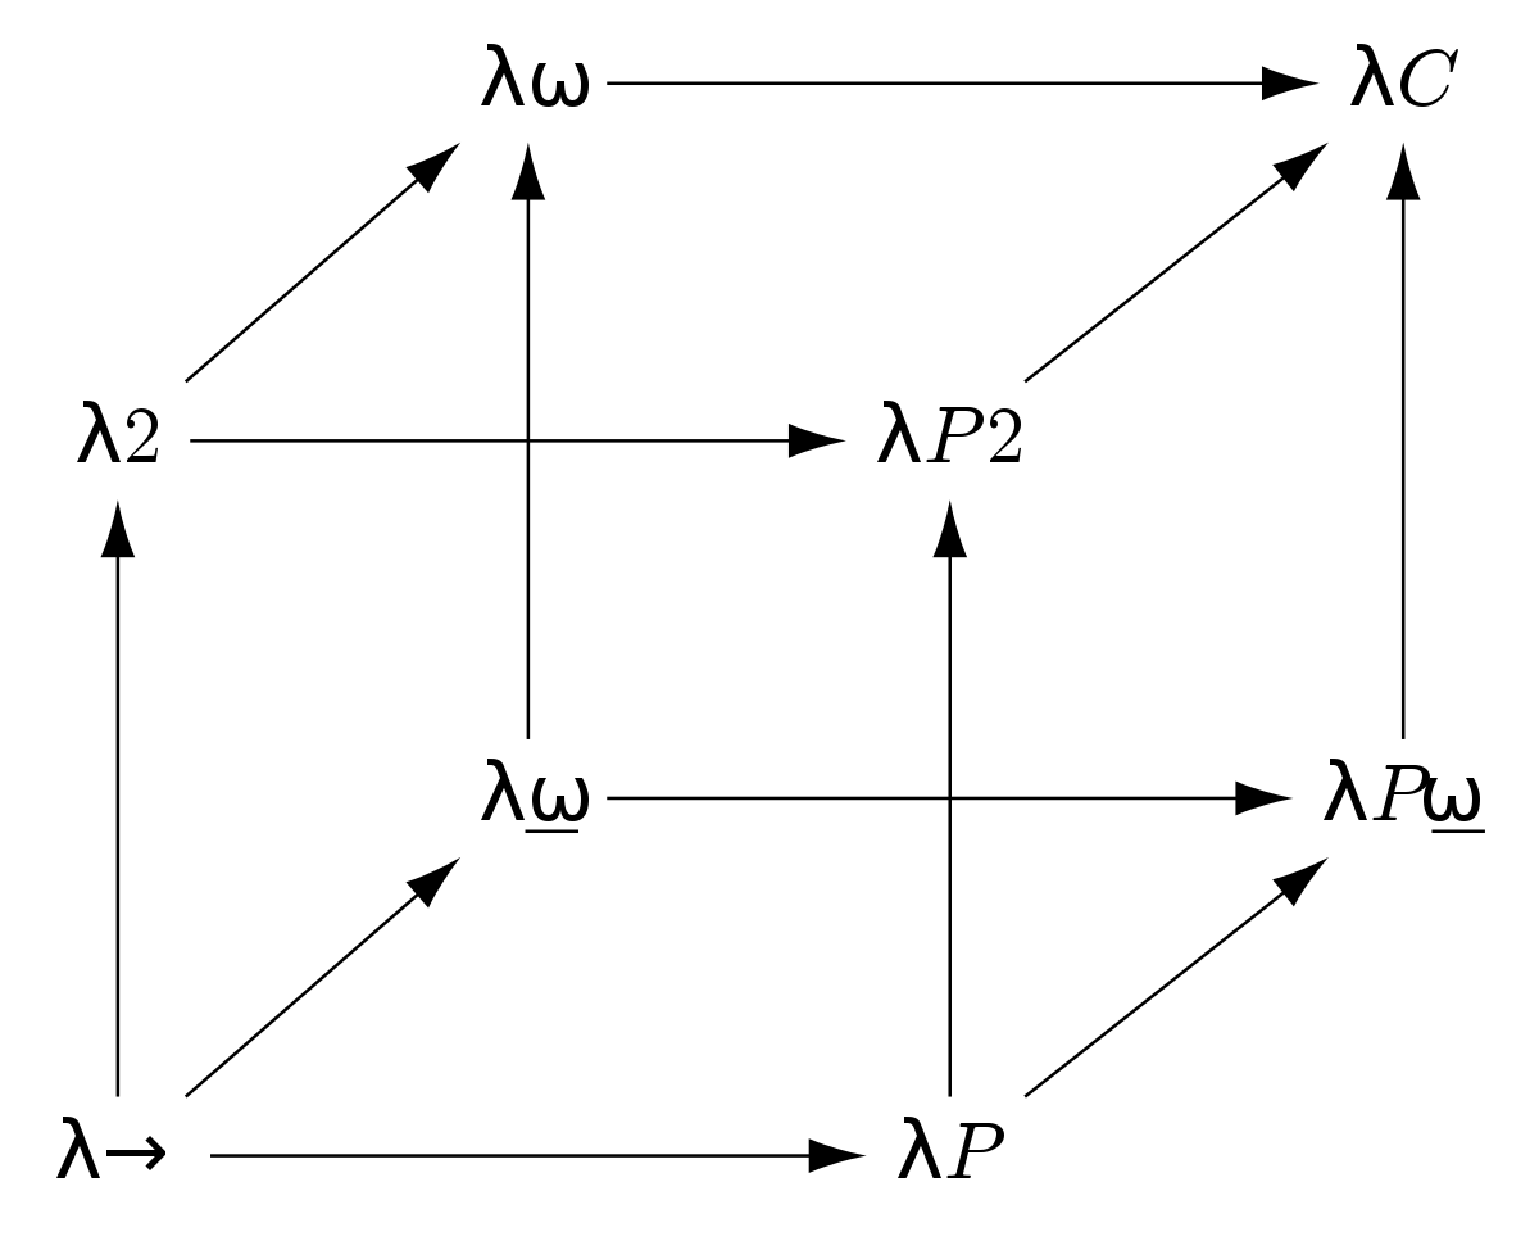
\includegraphics[width=3cm]{1200px-Lambda_Cube_img}
\caption{The lambda cube by Henk Barendregt.}
\label{fig:lambda_cube}
\end{figure}

But the biggest benefit of dependent types is the possibility to formulate constructive proofs about the desired properties of the program directly in it.
If the need for safe and secure software continues to increase as it did in the past, the need for dependent types will likely increase as well.
It is not realistic that every software developer will use dependent types, however, it can be of great advantage to know that dependent types exists as well as the basics of the concept.

As the concept of dependent types directly relates to the lambda calculus most of the currently known implementations are found in functional languages.
In this publication, all concrete code examples are based on Agda, as there are different beginner-friendly tutorials available as well as literature related to dependent types. Amogst others this includes "Dependently Typed Programming in Agda" from Ulf Norell \cite{norell:deptyped}, "Programming Languages Foundations in Agda" from Phil Wadler \cite{plfa2019} as well as "Verified Functional Programming in Agda" from Aaron Stump \cite{10.1145/2841316} on which most of the examples are based\footnote{A comprehensive list can be found in the documentation of Agda \cite{AgdaReadTheDocs}}.

A short introduction to Agda can be found in the following section \ref{section:first_steps_in_agda}.

Basic knowledge of lambda calculus as well as any functional programming language, such as Haskell, is recommended to benefit the most from the following sections.
